\chapter{Volumes of Common Solids}
\section{Rectangular Prism}
The volume of a rectangular solid is the product of its three
dimensions. If a block of ice is 5 cm tall, 3 cm wide, and 2 cm
deep, its volume is $5 \times 3 \times 2 = 30$ cubic centimeters.

\begin{mdframed}[style=important, frametitle={Volume of a rectangular solid.}]

A rectangular solid with height $h$, width $w$ and length/depth $l$ has volume:
$$V = lwh$$
\end{mdframed}

\tdplotsetmaincoords{80}{130} 
\begin{tikzpicture} [scale=1, tdplot_main_coords, axis/.style={->,sdkblue}, 
light vector/.style={-stealth,dashed,very thick, black}, 
vector/.style={-stealth,black,very thick}, 
vector guide/.style={dashed,sdkblue}]

%standard tikz coordinate definition using x, y, z coords
\coordinate (O) at (0,0,0);

%draw axes
\draw[axis] (0,0,0) -- (3,0,0) node[anchor=north east]{$x$};
\draw[axis] (0,0,0) -- (0,4,0) node[anchor=north west]{$y$};
\draw[axis] (0,0,0) -- (0,0,5.2) node[anchor=south]{$z$};

%draw a vector from O to P
\draw[thick,black] (0,0,0) -- (0,0,5);
\draw[thick,black] (0,3,5) -- (0,0,5);
\draw[thick,black] (2,0,5) -- (0,0,5);

\draw[thick,black] (0,0,0) -- (0,3,0);
\draw[thick,black] (0,3,5) -- (0,3,0) node[midway, right]{$5$ cm};
\draw[thick,black] (2,3,0) -- (0,3,0) node[midway, below]{$2$ cm};;

\draw[thick,black] (0,0,0) -- (2,0,0);
\draw[thick,black] (2,0,5) -- (2,0,0);
\draw[thick,black] (2,3,0) -- (2,0,0) node[midway,below]{$3$ cm};

\draw[thick,black] (2,3,5) -- (2,0,5);
\draw[thick,black] (2,3,5) -- (0,3,5);
\draw[thick,black] (2,3,5) -- (2,3,0);

\end{tikzpicture}


A
cubic centimeter is the same as a milliliter. A milliliter of ice
weighs about 0.92 grams.  This means the block of ice would have a mass of $30
\times 0.92 = 27.6$ grams. \index{volume ! rectangular solid}
\section{Triangular Prism}\index{volume ! triangular prism}
Triangular prisms are 3D versions of triangles (imagine stretching a triangle out of the page). 
It has 2 triangular faces and 3 rectangular faces.
\begin{mdframed}[style=important, frametitle={Volume of a triangular prism.}]
Recall the area of a triangle is $V=\frac{1}{2}wh$ where w is the width or base and h is the height of the triangle.
A triangular prism with height $h$, width $w$ and length/depth $l$ has volume:
$$V = \frac{1}{2}lwh$$
\end{mdframed}

%FIXME image is basic, match with other format
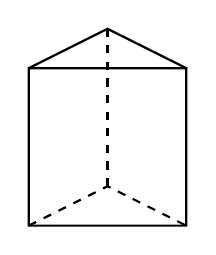
\begin{tikzpicture}
 \draw[dashed,thick] (-1,0) -- (0,0.5) edge (0,2.5) -- (1,0);
 \draw[thick] (-1,0) rectangle (1,2) -- (0,2.5) -- (-1,2);
\end{tikzpicture}

\section{Spheres}
\begin{mdframed}[style=important, frametitle={Volume of a Sphere}]

A sphere with a radius of $r$ has a volume of \index{volume ! sphere}

$$v = \frac{4}{3} \pi r^3$$

(For completeness, the surface area of that sphere would be

$$a  = 4 \pi r^2$$

Note that a circle of radius $r$ is one quarter of this: $\pi r^2$.)

\end{mdframed}

\begin{Exercise}[title={Flying Sphere}, label=flying_sphere]

An iron sphere is traveling at 5 m/s (and is not spinning).  The
sphere has a radius of 1.5 m.  Iron has a density of 7,800 kg per
cubic meter.  How much kinetic energy does the sphere have?
\end{Exercise}
\begin{Answer}[ref=flying_sphere]
  The volume of the sphere (in cubic meters) is

  $$\frac{4}{3}\pi (1.5)^3 = 4.5 \pi \approx 14.14$$

  The mass (in kg) is $14.14 \times 7800 \approx 110,269$

  The kinetic energy (in joules) is

  $$k = \frac{110269 \times 5^2}{2} = 1,378,373$$

  About 1.4 million joules.
\end{Answer}

\section{Cylinders}

The base and the top of a right cylinder are identical circles. The
circles are on parallel planes.  The sides are perpendicular to those
planes.

\tdplotsetmaincoords{75}{0} 
\begin{tikzpicture} [scale=4, tdplot_main_coords, axis/.style={->,sdkblue}]
\draw[dashed, sdkblue] (0.5,0,0) -- (0.5,0,0.7) node[midway, right]{$h$};
\draw[dashed, sdkblue] (0.5,0,0) -- (1,0,0) node[midway, below]{$r$};
\draw[black] (0.5, 0, 0) circle (0.5);
\draw[black] (0.5, 0, 0.7) circle (0.5);
\draw[black] (0,0,0) -- (0,0,0.7);
\draw[black] (1,0,0) -- (1,0,0.7);
\draw[black] (0.5,0,0) circle (0.02);
\draw[black] (0.5,0,0.7) circle (0.02);
\end{tikzpicture}

\begin{mdframed}[style=important, frametitle={Volume of a cylinder}]\index{volume ! right cylinder}


The volume of the right cylinder of radius $r$ and height
$h$ is given by:

$$v = \pi r^2 h$$

In other words, it is the area of the base times the height.

\end{mdframed}

\begin{Exercise}[title={Tablet}, label=tablet]

  A drug company needs to create a tablet with volume of 90 cubic millimeters.

  The tablet will be a cylinder with half spheres on each end.  The radius will be 2mm.

  How long do they need to make the tablet to be?

  \vspace{2mm}
  
\tdplotsetmaincoords{90}{20} 
\begin{tikzpicture} [scale=6.5, tdplot_main_coords, axis/.style={->,sdkblue}]
\draw[dashed, sdkblue] (-0.2,0,0) -- (0,0,0);
\draw[dashed, sdkblue] (0,0,0) -- (0,0,0.2) node[midway, right]{2 mm};
\draw[dashed, sdkblue] (0, 0, 0) [x={(0,0,1)}] circle (0.2);
\draw[dashed, sdkblue] (0.5, 0, 0) [x={(0,0,1)}] circle (0.2);
\draw[dashed, sdkblue] (0.5,0,0) -- (0.7,0,0);
\draw[black] (0, 0, -0.2) [y={(0,0,-1)}] arc (90:270:0.2);
\draw[black] (0.5, 0, 0.2) [y={(0,0,-1)}] arc (-90:90:0.2);
\draw[black] (0,0,0.2) -- (0.5,0,0.2);
\draw[black] (0,0,-0.2) -- (0.5,0,-0.2);
\draw[dashed, sdkblue] (-0.2, 0, 0) -- (-0.2, 0, -0.3);
\draw[dashed, sdkblue] (0.7, 0, 0) -- (0.7, 0, -0.3);
\draw[dashed, sdkblue] (-0.2, 0, -0.3) -- (0.7, 0, -0.3) node[midway, below]{?};
\end{tikzpicture}
  

\end{Exercise}
\begin{Answer}[ref=tablet]
  In your mind, you can disassemble the tablet into a sphere (made up of
  the two ends) and a cylinder (between the two ends).
  
  The volume of the sphere (in cubic millimeters) is

  $$\frac{4}{3}\pi (2)^3 =\frac{32}{3}\pi \approx 33.5$$

  Thus, the cylinder part has to be $90 - 33.5 = 56.5$ cubic mm. The
  cylinder part has a radius of 2 mm. If the length of the cylinder
  part is $x$, then

  $$\pi 2^2 x = 56.5$$

  Thus $x = \frac{56.5}{4 \pi} \approx 4.5$ mm.

  The cylinder part of the table needs to be 4.5mm.  Thus the entire tablet is 8.5mm long.
  
\end{Answer}

What if the base and top are identical, but the sides aren't
perpendicular to the base? This is called \newterm{oblique cylinder}.

\tdplotsetmaincoords{75}{0} 
\begin{tikzpicture} [scale=4, tdplot_main_coords, axis/.style={->,sdkblue}]
\draw[dashed, sdkblue] (0.7,0,0) -- (0.7,0,0.7) node[midway, right]{$h$};
\draw[dashed, sdkblue] (0.5,0,0) -- (1,0,0) node[midway, below]{$r$};
\draw[black] (0.5, 0, 0) circle (0.5);
\draw[black] (0.7, 0, 0.7) circle (0.5);
\draw[black] (0,0,0) -- (0.2,0,0.7);
\draw[black] (1,0,0) -- (1.2,0,0.7);
\draw[black] (0.5,0,0) circle (0.02);
\draw[black] (0.7,0,0.7) circle (0.02);
\end{tikzpicture}

The volume is still the height times the area of the base.  Note,
however, that the height is measured perpendicular to the bottom and
top. \index{volume ! oblique cylinder}

Why is this the case?


\section{Pyramids}

On a solid with a flat base, the line that we use to measure height is
always perpendicular to the plane of the base. We can take slices
through the solid that are parallel to that base plane.  For example,
if we have a pyramid with a square base, each slice will be a square
--- small squares near the top, larger squares near the bottom. 
The sides of the pyramids are all triangles, so these are referred to as Triangular Pyramids, just pyramids, or sometimes, Tetrahedrons.
\tdplotsetmaincoords{80}{17} 
\begin{tikzpicture} [scale=4, tdplot_main_coords, axis/.style={->,sdkblue}]
  
\draw[dashed, sdkblue] (0.5,0.5,0) -- (0.5,0.5, 1.0) node[midway, right]{$h$};

\draw[black] (0,0,0) -- (0.5,0.5,1.0);
\draw[black] (1,0,0) -- (0.5,0.5,1.0);
\draw[black] (0,1,0) -- (0.5,0.5,1.0);
\draw[black] (1,1,0) -- (0.5,0.5,1.0);

\draw[black] (0,0,0) -- (1,0,0);
\draw[black] (0,0,0) -- (0,1,0);
\draw[black] (1,0,0) -- (1,1,0)node[midway,below]{$w$};
\draw[black] (0,1,0) -- (1,1,0);

\fill[sdkblue,,opacity=0.4] (0.125, 0.125, 0.25) -- (0.875, 0.125, 0.25) -- (0.875, 0.875, 0.25) -- (0.125, 0.875, 0.25);

\draw[dashed,sdkblue] (0.125, 0.125, 0.25) -- (0.875, 0.125, 0.25);
\draw[dashed,sdkblue] (0.125, 0.125, 0.25) -- (0.125, 0.875, 0.25);
\draw[dashed,sdkblue] (0.875, 0.125, 0.25) -- (0.875, 0.875, 0.25);
\draw[dashed,sdkblue] (0.125, 0.875, 0.25) -- (0.875, 0.875, 0.25);

\draw[dashed,sdkblue] (-0.1, -0.1, 0.25) -- (1.1, -0.1, 0.25);
\draw[dashed,sdkblue] (-0.1, -0.1, 0.25) -- (-0.1, 1.1, 0.25);
\draw[dashed,sdkblue] (1.1, -0.1, 0.25) -- (1.1, 1.1, 0.25);
\draw[dashed,sdkblue] (-0.1, 1.1, 0.25) -- (1.1, 1.1, 0.25);

\end{tikzpicture}

We can figure out the area of the slice at every height $z$.  For
example, at $z = 0$, the slice would have area $w^2$.  At $z = h$, the
slice would have zero area.  What about an arbitrary $z$ in between?
The edge of the square would be $w (1 - \frac{z}{h})$.  The area of
the slice would be $w^2 (1 - \frac{z}{h})^2$

The graph of this would look like this:

\begin{tikzpicture}[scale=5]

\draw [sdkblue,->,thick] (0,0) -- (1.1,0) node[right]{$z$};
\draw [sdkblue,->,thick] (0,0) -- (0,1.1) node[above]{slice area};
\draw [sdkblue,dashed] (1, 1) -- (0,1) node[left] {$w^2$};
\draw [sdkblue,dashed] (1, 1) -- (1,0) node[below] {$h$};
 \fill [sdkblue, opacity=0.4, domain=0:1, variable=\x]
      (0, 0) 
      -- plot ({\x}, {(1.0 - \x)^2})
      -- (1, 0)
      -- cycle;
\draw[thick,draw=black,
      domain=0:1,samples=300,variable=\x] 
      plot (\x,{(1.0 - \x)^2});
\end{tikzpicture}

The volume is given by the area under the curve and above the
axis. Once you learn integration, you will be extra good at finding
the area under the curve.  In this case, we will just tell you that the colored region in the picture is one third of the rectangle.

Thus, the area of a square-based pyramid is $\frac{1}{3} h w^2$.

In fact:

\begin{mdframed}[style=important, frametitle={Volume of a pyramid}]\index{volume ! pyramid}

  The volume of pyramid whose base has an area of $b$ and height $h$ is given by:

  $$V = \frac{1}{3} h b$$

  Regardless of the shape of the base.
\end{mdframed}

Note that this is true even for oblique pyramids:

\tdplotsetmaincoords{80}{30} 
\begin{tikzpicture} [scale=4, tdplot_main_coords, axis/.style={->,sdkblue}]
  
\draw[dashed, sdkblue] (1.6,0.5,0) -- (1.6,0.5, 1.0) node[midway, right]{$h$};
\fill[sdkblue] (1.6, 0.5, 0) circle (.02);

\draw[black] (0,0,0) -- (1.6,0.5,1.0);
\draw[black] (1,0,0) -- (1.6,0.5,1.0);
\draw[black] (0,1,0) -- (1.6,0.5,1.0);
\draw[black] (1,1,0) -- (1.6,0.5,1.0);

\draw[black] (0,0,0) -- (1,0,0);
\draw[black] (0,0,0) -- (0,1,0);
\draw[black] (1,0,0) -- (1,1,0);
\draw[black] (0,1,0) -- (1,1,0);

\fill[sdkblue,opacity=0.4] (0.4, 0.125, 0.25) -- (1.15, 0.125, 0.25) -- (1.15, 0.875, 0.25) -- (0.4, 0.875, 0.25);

\draw[dashed,sdkblue] (0, -0.1, 0.25) -- (1.3, -0.1, 0.25);
\draw[dashed,sdkblue] (0, -0.1, 0.25) -- (0, 1.1, 0.25);
\draw[dashed,sdkblue] (1.3, -0.1, 0.25) -- (1.3, 1.1, 0.25);
\draw[dashed,sdkblue] (0, 1.1, 0.25) -- (1.3, 1.1, 0.25);

\end{tikzpicture}


\begin{Exercise}[title={Hexagon-based Pyramid}, label=pyramid_volume]

There is a pyramid with a regular hexagon for a base. Each edge is 5 cm long.  The pyramid is 13 cm tall.  What is its volume?

\tdplotsetmaincoords{70}{17} 
\begin{tikzpicture} [scale=.5, tdplot_main_coords]
  
\draw[dashed, sdkblue] (0,0,0) -- (0,0,13) node[right]{13 cm};

\draw[black] (-5,0,0) -- (-2.5,4.33,0) -- (2.5,4.33,0) -- (5,0,0)
-- (2.5, -4.33, 0) -- (-2.5, -4.33,0) -- cycle;

\draw[black] (0, -4.5, 0) node {5 cm};

\draw[black] (-5,0,0) -- (0,0,13);
\draw[black] (0,0,13)--(5,0,0);
\draw[black] (-2.5,4.33,0) -- (0,0,13);
\draw[black] (2.5,4.33,0) -- (0,0,13);
\draw[black] (-2.5,-4.33,0) -- (0,0,13);
\draw[black] (2.5,-4.33,0) -- (0,0,13);
\end{tikzpicture}

\end{Exercise}
\begin{Answer}[ref=pyramid_volume]
  First, you need to find the area of the base, which is a regular hexagon:
  
\begin{tikzpicture}[scale=0.5]
  \draw[black] (-5,0) -- (-2.5,4.33) -- (2.5,4.33) -- (5,0)
-- (2.5, -4.33) -- (-2.5, -4.33) -- cycle node[midway,left]{5 cm};
\draw[sdkblue,dashed] (-5,0) -- (0,0);
\draw[sdkblue,dashed] (5,0) -- (0,0);
\draw[sdkblue,dashed] (-2.5,4.33) -- (0,0);
\draw[sdkblue,dashed] (2.5,4.33) -- (0,0);
\draw[sdkblue,dashed] (-2.5,-4.33) -- (0,0);
\draw[sdkblue,dashed] (2.5,-4.33) -- (0,0);
\end{tikzpicture}

All the angles in this picture are $60^\circ$ or $\frac{\pi}{3}$
radians. This means each line is 5 cm long.

This tells us that we need to find the area of one of these triangles and multiply that by six.

Every triangle has a base of 5cm. How tall are they?

\begin{tikzpicture}
  \draw[black] (-2.5,0) -- (2.5,0) -- (0,4.33) -- cycle node[midway,left]{5 cm};
  \draw[sdkblue,dashed] (0,0) -- (0,4.33) node[midway,right]{?};
  \draw[black] (-2.0, 0.0) node [right, above] {$60^\circ$};
\end{tikzpicture}

$$5 \sin{60^\circ} = 5\frac{\sqrt{3}}{2}$$

Which is about 4.33 cm.

So, the area of single triangle is 

$$\frac{1}{2} (5) \left( 5\frac{\sqrt{3}}{2} \right) = 25 \frac{\sqrt{3}} {4}$$

And the area of the whole hexagon is six times that:

$$75 \frac{\sqrt{3}}{2}$$

Thus, the volume of the pyramid is:

$$\frac{1}{3}h b = \frac{1}{3} 13 \left(75 \frac{\sqrt{3}}{2}\right)$$

About 281.46 cubic centimeters.

\end{Answer}

Note that plotting the area of each slice and finding the area under
the curve will let you find the area of many things.  For example,
let's say that you have a four-sided spiral, where each face has the
same width $w$:

\tdplotsetmaincoords{80}{17} 
\begin{tikzpicture} [scale=4, tdplot_main_coords, axis/.style={->,sdkblue}]

  \def\h{1.570796326794897}
  \def\gap{0.2}
  \def\srad{0.707106781186548}

\fill[sdkblue,opacity=.7] (0,-1,0) -- (-1,0,0) -- (0,1,0) -- (1,0,0) -- cycle;

\draw[black,thick] (0,-1,0) -- (-1,0,0) -- (0,1,0) -- (1,0,0) -- cycle;
\draw[black,thick] (0,-1,\h) -- (-1,0,\h) -- (0,1,\h) -- (1,0,\h) -- cycle;

\foreach \x in {0.0, 0.1, 0.2, 0.3, 0.4, 0.5, 0.6, 0.7, 0.8, 0.9, 1.0, 1.1, 1.2, 1.3, 1.4, 1.5}{
%        \fill[sdkblue, opacity=0.3] ({sin(deg(\x) + 0)},{cos(deg(\x)+ 0)},\x) -- ({sin(deg(\x) + 90)},{cos(deg(\x)+ 90)},\x) --
%        ({sin(deg(\x + \gap) + 90)},{cos(deg(\x + \gap) + 90)},\x + \gap) -- ({sin(deg(\x + \gap) + 0},{cos(deg(\x + \gap)+ 0)},\x + \gap) -- cycle;
        
%        \fill[gray, opacity=0.8] ({sin(deg(\x) + 90)},{cos(deg(\x)+ 90)},\x) -- ({sin(deg(\x) + 180)},{cos(deg(\x)+ 180)},\x) --
%        ({sin(deg(\x + \gap) + 180)},{cos(deg(\x + \gap)+ 180)},\x + \gap) -- ({sin(deg(\x + \gap) + 90)},{cos(deg(\x + \gap)+ 90)},\x + \gap) -- cycle;
        
%        \fill[sdkblue,opacity=0.3] ({sin(deg(\x) + 180)},{cos(deg(\x)+ 180)},\x) -- ({sin(deg(\x) + 270)},{cos(deg(\x)+ 270)},\x) --
%        ({sin(deg(\x + \gap) + 270)},{cos(deg(\x + \gap)+ 270)},\x+\gap) -- ({sin(deg(\x + \gap) + 180)},{cos(deg(\x + \gap)+ 180)},\x + \gap) -- cycle;
        
%        \fill[gray] ({sin(deg(\x) + 270)},{cos(deg(\x)+ 270)},\x) -- ({sin(deg(\x) + 0)},{cos(deg(\x)+ 0)},\x) --
  %        ({sin(deg(\x + \gap) + 0)},{cos(deg(\x + \gap)+0)},\x + \gap) -- ({sin(deg(\x + \gap) + 270)},{cos(deg(\x + \gap)+ 270)},\x +\gap) -- cycle;

  \draw[sdkblue] ({sin(deg(\x) + 0)},{cos(deg(\x)+ 0)},\x) -- ({sin(deg(\x) + 90)},{cos(deg(\x)+ 90)},\x) --
  ({sin(deg(\x) + 180)},{cos(deg(\x)+ 180)},\x) -- ({sin(deg(\x) + 270)},{cos(deg(\x)+ 270)},\x);
      }

\draw[thick,draw=black,
      domain=0:\h,samples=100,variable=\x] 
      plot ({sin(deg(\x) + 0)},{cos(deg(\x)+ 0)}, \x);

\draw[dashed,draw=sdkblue,
      domain=0:\h,samples=100,variable=\x] 
      plot ({\srad * sin(deg(\x) + 45)},{\srad * cos(deg(\x)+ 45)}, \x);

\draw[thick,draw=black,
      domain=0:\h,samples=100,variable=\x] 
      plot ({sin(deg(\x) + 90)},{cos(deg(\x)+ 90)}, \x);
\draw[dashed,draw=sdkblue,
      domain=0:\h,samples=100,variable=\x] 
      plot ({\srad * sin(deg(\x) + 135)},{\srad * cos(deg(\x)+ 135)}, \x);
      
\draw[thick,draw=black,
      domain=0:\h,samples=100,variable=\x] 
      plot ({sin(deg(\x) + 180)},{cos(deg(\x) + 180)}, \x);
%\draw[dashed,draw=sdkblue,
%      domain=0:\h,samples=100,variable=\x] 
%      plot ({\srad * sin(deg(\x) + 225)},{\srad * cos(deg(\x)+ 225)}, \x);

      
\draw[dashed, thick,draw=black,
      domain=0:\h,samples=100,variable=\x] 
      plot ({sin(deg(\x) + 270)},{cos(deg(\x) + 270)}, \x);

%\draw[dashed,draw=sdkblue,
%      domain=0:\h,samples=100,variable=\x] 
%      plot ({\srad * sin(deg(\x) + 315)},{\srad * cos(deg(\x)+ 315)}, \x);


      \fill[sdkblue,opacity=.9] (0,-1,\h) -- (-1,0,\h) -- (0,1,\h) -- (1,0,\h) -- cycle;
      \draw (0.7,-0.6,0) node [below] {$w$};
      \draw[dashed, sdkblue] (-1.1,0,0) -- (-1.1,0,\h) node[midway,left]{$h$};


\end{tikzpicture}

Every slice still has an area of $w^2$,  which means this figure has a volume of $h w^2$.


\begin{Exercise}[title={Volume of a building}, label=building_volume]

An architect is designing a hotel with a right triangular base; the base is 30
meters on each leg.  The building gets narrower as you get closer to
the top, and finally shrinks to a point.  The spine of the building is
where the right angle is. That spine is straight and perpendicular to the ground.

Each floor has a right isosceles triangle as its floor plan.  The
length of each leg is given by this formula:

$$w = 30 \sqrt{1 - \frac{z}{100}}$$

So, the width of the building is 30 meters at height $z=0$.  At 100
meters, the building comes to a point.  It will look like this:
\hspace{8mm}

\tdplotsetmaincoords{75}{120}
\begin{tikzpicture} [scale=1, tdplot_main_coords]
\def\h{10}
\draw[dashed, sdkblue] (0,3,0) -- (0,3.2,0) -- (0,3.2,\h) node[midway, right]{100m} -- (0,0,\h);

\draw[black] (0,0,0) -- (3,0,0) -- (0,3,0) -- cycle node [midway, above]{30m};
\draw[black] (0,0,0) -- (0,0,\h);
\draw[black] (0.5, 0, 0) -- (0.5, 0.5, 0) -- (0, 0.5, 0);
\draw[thick,draw=black,
      domain=0:\h,samples=100,variable=\x] 
      plot ({3 * sqrt(1 - (\x/\h)}, 0, \x);

\draw[thick,draw=black,
      domain=0:\h,samples=100,variable=\x] 
      plot (0, {3 * sqrt(1 - (\x/\h))}, \x);

\foreach \n in {1,...,\h}{
  \draw [dashed, draw=sdkblue] (0,0,\n) -- ({3 * sqrt(1 - \n/\h)}, 0, \n) -- (0, {3 * sqrt(1 - \n/\h)},\n) -- cycle;
  \draw [draw=sdkblue] (0.5,0,\n) -- (0.5, 0.5, \n) -- (0, 0.5,\n);
};
      
\end{tikzpicture}

What is the volume of the building in cubic meters?
\end{Exercise}
\begin{Answer}[ref=building_volume]

  The area at height $z$ is given by:

  $$a = \frac{1}{2} w^2 =\frac{1}{2} \left(30 \sqrt{1 - \frac{z}{100}}\right)^2 = \frac{1}{2} 900 \left(1 - \frac{z}{100}\right)$$

  If we plot that, it looks like this:

\begin{tikzpicture}
  \def\h{5}
  \draw[sdkblue, ->] (0,0) -- (0, \h + 0.5) node[above] {area};
  \draw[sdkblue, ->] (0,0) -- (3.5, 0) node[right] {$z$};
 \fill [sdkblue, opacity=0.4]
      (0, 0) -- (0,\h) node [left] {$900 m^2$} -- (3,0) node[below] {$100 m$} -- cycle;
\end{tikzpicture}

What is the area of the blue region? $\frac{1}{2} (900)(100) = 45,000$

The building will be 45 thousand cubic meters.


\end{Answer}
% FIXME
% volume of ellipse? 
% and cone since it is included in quiz questions and heavily in the next chapter